\section{Theta Sketches}
\label{sec:theta}

Our first example is a $\Theta$ sketch implemented using  the 
\emph{K Minimum Values  (KMV)} algorithm~\cite{KMV}, 
which estimates the number of unique items in a data stream. 
We first overview the sequential  sketch in Section~\ref{ssec:theta-overview}, 
and then explain how we parallelize it in Section~\ref{ssec:concurrent-theta}.
Section~\ref{ssec:theta-analysis} analyzes the algorithm's correctness and error bounds.

\subsection{Overview}
\label{ssec:theta-overview}


A $\Theta$ sketch maintains a set of samples and a parameter $\Theta$
that determines which elements are added to the sample set. 
It uses a random hash function whose outputs are uniformly distributed
in the range $[0,1]$, and $\Theta$ is always in the same range.  
Every incoming data stream element is first hashed, and then the hash is compared to $\Theta$. 
In case it is smaller, the value is added to the sample set.  Otherwise, it is ignored. 

Because the hash outputs are uniformly distributed, an expected
portion $\Theta$ of them are smaller than $\Theta$ and hence included in the sample. 
Therefore, we can estimate the number of unique data items in the stream by
simply dividing the number of (unique) stored samples by $\Theta$.
The error depends on the size of the sample set -- with $K$ samples, 
the  >
Note that 
this analysis assumes that the random hash function is drawn independently of the stream values.

 $\Theta$ sketches keep constant-size sample sets, independently of the stream size. 
 To this end, they need to adjust $\Theta$ on-the-fly, and prune elements of 
 the sample set whose hashes are smaller than the new $\Theta$.
%There are a number of approaches to do that. 
A straightforward KMV solution keeps a sample of size $K$ 
holding the  values with the $K$ smallest hashes seen so far. 
In this case $\Theta$ is $1$ during the first $K$ updates, and 
subsequently it is the hash of the largest sample in the set.
Once the sample set is full,
every update that inserts  a new element also removes the largest
element in the set and updates $\Theta$ accordingly. 
This can be implemented efficiently by keeping the samples in  a min-heap. 
A nice property of this KMV variant is that it is \emph{order agnostic}, i.e., produces 
identical results for streams that consist of the same elements albeit in a different order.

\inblue{ [[Let's try to replace quickselect by the straightforward variant in the experiments and remove this discussion. ]]
The slightly optimized \emph{quickselect} variant of KMV keeps samples 
in a hashmap, and  allows the sample size to vary between $K$ and $2K$
as illustrated in  Figure~\ref{fig:thetaSampling}.
Insertions are quicker as long as the hash does not overflow, and once
it does (i.e., includes $2K$ samples), the algorithm uses quickselect to 
find the $K^{th}$ smallest value and deletes all bigger values. 
This variant is not order agnostic, because the order in which elements appear can impact how many 
elements end up being sampled.
Note that since typically, $K \ll n$, the vast majority of hashes are larger than 
$\Theta$,  and so most update operations complete without updating the sample set. 
Therefore, the impact of this optimization is not dramatic. 
} 

\begin{figure}[H]
    \centering
    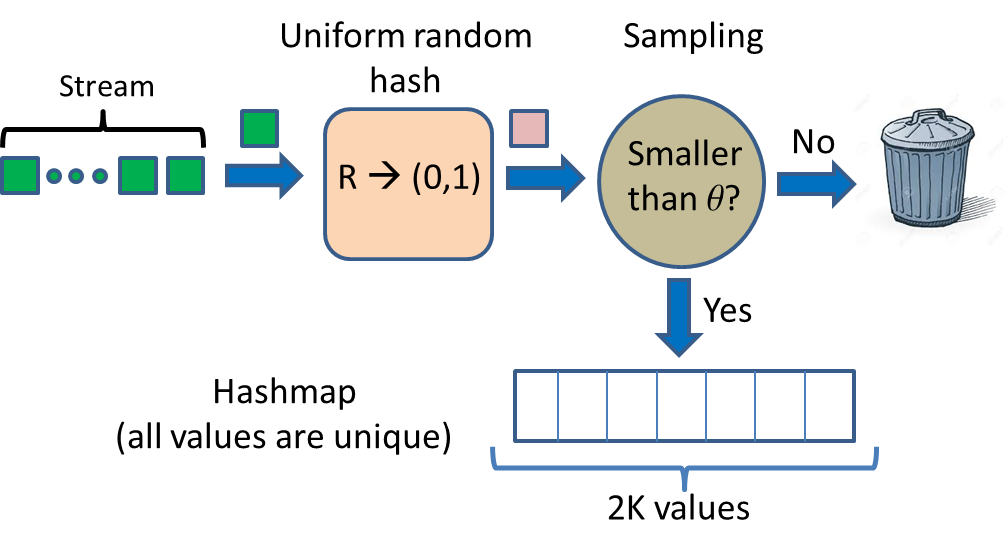
\includegraphics[width=2.5in]{images/thetaSampling.png}
    \caption{Sampling in quickselect KMV algorithm. \inred{I have many issues with this picture: (1) Fonts are too small. 
    (2) What is the R in the hash box? Please remove. 
    (3) The hashmap has 2K entries (not lower case k, not values). (4) Ifs in flowcharts are diamonds, not circles.
    (5) There is a missing diamond ``hash full?'' with pruning of the map and update of $\Theta$ in case of yes.
    Of course all this is only relevant if we decide to keep this algorithm.}}
    \label{fig:thetaSampling}
\end{figure}





\subsection{Concurrent algorithm}
\label{ssec:concurrent-theta}

%As mentioned in Section~\ref{sub:concurency}, 
Our concurrent implementation -- given in  Algorithm~\ref{alg:concurrent-theta} 
and illustrated in Figure~\ref{fig:concurrentTheta} --  
uses multiple threads to process incoming stream elements; 
it services queries at any time during the sketch's construction. 
%Since the only thing threads need to know in order to sample stream elements is
%the value of $\Theta$, they can do so locally in parallel, 
Update threads sample stream elements in parallel into local buffers, 
while a background thread periodically propagates the sampled values to a shared sketch
consisting of sampleSet and $\Theta$. 


\begin{algorithm}[tb]
\small
\begin{multicols}{2}
\begin{algorithmic}[1]

%\State {\bf Sketch variables:}
\Vars
\State   sampleSet, init $\emptyset$ \Comment global samples
\State  $\Theta$, init $1$			\Comment global threshold
\State {\tt atomic} est, init $0$ \Comment estimated \# uniques
\State $h$, init random uniform hash function 
\Statex
\ForEach{update thread $t_i$} 
	\State \emph{buf$_i$}, init $\emptyset$ \Comment local sample set
	\State \emph{aux$_i$}, init $[ ]$ \Comment auxiliary array
	\State $\Theta_i$, init $1$ 	\Comment local threshold
	\State {\tt atomic} $P_i$, init $1$ \Comment for synchronization
\EndFor
\EndFor

\Statex
\Procedure{query}{}
\State return est \label{l:query}
\EndProcedure
%\Statex

\Procedure{update$_i$}{val}
\If{$h$(val) $< \Theta_i$} 
	add val to \emph{buf$_i$} \label{l:local-sample}
\EndIf
\If{$|$\emph{buf$_i$}$| > b$} \Comment propagate
	\State wait until $P_i >0$ \label{l:wait}
	\State $\Theta_i \leftarrow P_i$ \label{l:adopt}
	\State \emph{aux$_i$}  $\leftarrow$ sort by $h$ $\{ e \in \mathit{buf_i} | h(e) <\Theta_i \}$
		\label{l:sort}
	\State $P_i \leftarrow 0$ 		\label{l:signal}
	\State \emph{buf$_i$}$ \leftarrow \emptyset$  \label{l:clean} 

\EndIf  
\EndProcedure

\Procedure{propagator}{}
\While {true}
\ForAll{update thread $t_i$ s.t. $P_i =0$} 
		\State  update sampleSet and $\Theta$ with \emph{aux$_i$} \label{l:aux}
		\State est $\leftarrow |$sampleSet$|/ \Theta$ \label{l:update-est}
		\State $P_i \leftarrow \Theta$  \label{l:theta}
\EndFor
\EndWhile
\EndProcedure

\end{algorithmic}
\end{multicols}
\caption{Concurrent $\Theta$ sketch algorithm.}
\label{alg:concurrent-theta}
\end{algorithm}

The key to achieving efficiency is exploiting locality and minimizing synchronization.
Every worker thread $t_i$ samples stream elements into a local bounded buffer 
\emph{buf$_i$} of size $b$ (line~\ref{l:local-sample}). 
To avoid frequent cache invalidations, $t_i$ uses a periodically refreshed
local copy $\Theta_i$ of $\Theta$. 
Because the global  $\Theta$ is monotonically decreasing, periodically copying it
into local copies maintains the invariant $\Theta_i \geq \Theta$.
Thus, while threads may over-sample, they never fail to sample elements that need 
to be included in the shared sketch. 
%Initially, all buffers are empty and all local $\Theta_i$s are $1$. 

When the buffer of a thread $t_1$ becomes full, $t_1$ sorts it
into an auxiliary array \emph{aux$_i$} and signals to the propagator  to union
it with the shared sketch (lines~\ref{l:sort}--\ref{l:signal}).
In the meantime, $t_1$ proceeds to re-fill its buffer with new samples.
The propagation  (line~\ref{l:aux}), in turn,  is highly optimized, as it merges a sorted array of 
values into the sampleSet, and can stop merging upon encountering 
an element whose hash is bigger than the global $\Theta$.

Update thread $t_i$ synchronizes with the propagator using a 
single \emph{atomic} variable $P_i$, which it sets to zero 
to signal to the propagator that the auxiliary array is ready.  
Because $P_i$ is  atomic, the Java memory model
guarantees that $t_i$'s auxiliary array is visible to
the background thread when $P_i$'s update is.
This is  an expensive operation (involving a memory fence),  
but we do it only once per $b$ items retained in the sample.

Before propagating its buffer, $t_i$ waits
until $P_i > 0$  (line~\ref{l:wait}); 
this indicates that the propagation of the previous \emph{aux}$_i$
 has completed, and  \emph{aux}$_i$ may
be reused. Thus, we  ensure that the sketch uses bounded space.
%
When the background thread completes the propagation, 
it piggybacks the global $\Theta$, which only it updates, on $P_i$  (line~\ref{l:theta}), 
and $t_i$ adopts it  (line~\ref{l:adopt}). Thus, update threads   learn $\Theta$ at no
additional synchronization cost. 

In order to support  fast concurrent reads, the shared sketch
maintains an atomic variable est, estimating the number of
 unique items seen so far by the propagator.
The background thread updates this variable after each propagation.
Again, because est is atomic, updating it involves a costly memory fence, which we amortize by performing it once per $b$ updates. 

For the $S$.union($S'$) operation (omitted from the code), 
we assume $S'$ is not undergoing any updates. 
The propagator thread puts its normal tasks on hold, 
 adopts the smaller $\Theta$ of the two sketches, merges their sampleSets while filtering elements according to the new $\Theta$, updates est, and resumes its 
 propagation tasks. Other operations (query and update) continue undisturbed.


\begin{figure}[H]
    \centering
    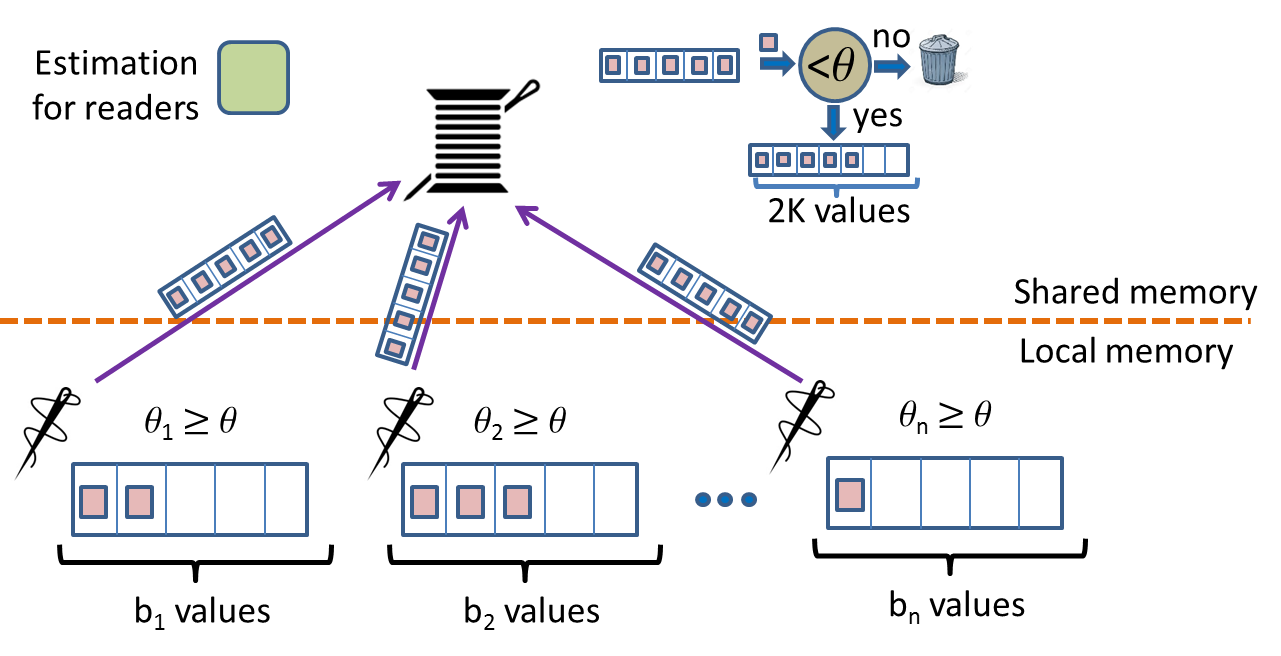
\includegraphics[width=4in]{images/thetaConcurrent.png}
    \caption{Concurrent $\Theta$ sketch architecture.
    \inred{Some requests for changes in the figure: 
    (1) Change $b_1$, $b_2$, and $b_3$ to $b$. 
    (2) Label the buffers as \emph{buf}$_1$ and \emph{aux}$_1$ etc. 
    (3) Write sort on one of the purple arrows. 
    (4) Replace 2K values with sampleSet.
    (5) remove the extra buffer on top, the aux buffered are merged directly into sampleSet. 
    (6) label the top thread as propagator.
    (7) Show a reader thread reading the estimate.
    (8) The classification of shared versus local memory is wrong. $\Theta$ and sampleSet are private
    	variables of the propagator.
    }}
    \label{fig:concurrentTheta}
\end{figure}

\subsection{Analysis}
\label{ssec:theta-analysis}

As explained above, we model the source of randomness used in the choice of $h$ as externally provided and the algorithm as  deterministic. We denote by $A^D_s$ the histories  of the deterministic sequential algorithm  (described in Section~\ref{ssec:theta-overview}) and by $A^r_s$ its $r$-relaxation. We denote by $A_c$ 
our (deterministic) concurrent algorithm (Algorithm~\ref{alg:concurrent-theta}).
%Section~\ref{ssec:concurrent-theta}).

When  $A_c$  uses $N$ update threads, its relaxation is $r=2Nb$. 
We first show that $A_c$  is strongly linearizable with respect to the relaxed specification $A^{2Nb}_s$,  and then analyze the error  of  $A^{2Nb}_s$.

\subsubsection{Strong linearizability wrt relaxed semantics}

For simplicity, we assume that lines  \ref{l:aux}--\ref{l:update-est} are executed atomically; 
in practice this assumption does not have any implications because $\Theta$ and sampleSet 
are private variables accessed only by the propagator.  

To prove correctness, we first show the following invariant about the samples maintained by 
our algorithm when using $N$ update threads.
\begin{invariant}[Sampling]
Consider a finite execution $\sigma$ of  $A_c$ and an update(v) that returns in $\sigma$. 
Then  at the end of $\sigma$,  if $h(v) < \Theta$ then 
$v\in \bigcup_{i=1}^N (\mathit{buf_i} \cup \mathit{aux_i}) \; \cup$ sampleSet.
\label{invariant:sampling}
\end{invariant}

\begin{proof}
The proof is by induction on the length of $\sigma$. The base for the empty execution is immediate. 
Now consider execution steps that can change the invariant.
First, consider an update that does not propagate \emph{buf$_i$}. 
Because each thread's $\Theta_i \le \Theta$ and a new update(v)  is sampled into \emph{buf$_i$} if 
$h(v) < \Theta_i$, the invariant is preserved.

Next, consider the propagation. 
In line~\ref{l:sort},  all elements of  \emph{buf$_i$}
whose hash value still exceeds $\Theta_i$ are inserted into \emph{aux$_i$} 
so clearing \emph{buf$_i$} in line~\ref{l:clean} preserves the invariant. 
It remains to show that when  \emph{aux$_i$} is overwritten in line~\ref{l:sort},
 all relevant entries from it have been propagated to  sampleSet (in line~\ref{l:aux}).
This is ensured by the atomic variable $P_i$, as follows:
(1) elements are added to \emph{aux$_i$} (line~\ref{l:sort}) only when $P_i >0$ while 
 the auxiliary thread propagates \emph{aux$_i$} into sampleSet according to $\Theta$ only when $P_i =0$,
 so \emph{aux$_i$} is never accessed concurrently by more than one thread;
(2) $P_i$ does not change from zero to non-zero unless  \emph{aux$_i$} has been propagated into sampleSet,
and is not overwritten by the update unless it changes from zero to non-zero. 
Finally, note that $\Theta$ is monotonically decreasing and previously sampled elements are removed from sampleSet only if their hashes exceed the new $\Theta$, again, preserving the invariant.
\end{proof}

Our strong linearizability proof uses two mappings,
$f$ and $g$,  from executions of $A_c$ to sequential executions. 
%
For an execution $\sigma$ of $A_c$,  $f(\sigma)$ is the sequential execution of $A_s$
consisting of  
operations invoked in $\sigma$,  ordered according to their invocation times. 
% when they execute their first step (line~\ref{l:query} for a query and~\ref{l:local-sample} for an update).
By definition, $f(\sigma)$ preserves the real-time order of $\sigma$ and $f$  is prefix-preserving.
To prove strong linearizability, it remains to show that $f(\sigma) \in A^{2Nb}_s$.

We define our second mapping, $g$, 
by ordering operations according to  \emph{visibility points} defined as follows: 
\begin{itemize}
\item
Visibility points of queries are their execution steps    (line~\ref{l:query}). 
%same as their linearization points. 
\item
For an update$_i$($v$) in $\sigma$, 
if $v$ is not added to \emph{buf$_i$} in line~\ref{l:local-sample}, then this point is its visibility point. 
%(as well as its linearization point). 
\item
Otherwise, consider an update$_i(v)$ that inserts $v$ into \emph{buf$_i$}, and  
let $t$ be the next time in $\sigma$ when thread $i$ propagates \emph{buf$_i$} into \emph{aux$_i$}
(i.e., executes line~\ref{l:sort}). The update's visibility point is 
the update of est (line~\ref{l:update-est}) that follows
the first propagation of \emph{aux}$_i$ into sampleSet (lines \ref{l:aux}--\ref{l:update-est})
after time $t$. 
\end{itemize}
 Note that in the latter case, 
the visibility point may occur after the update returns, and so $g$ does not 
necessarily preserve real-time order.

To complete the proof, we will show that for every execution $\sigma$ of $A_c$:
(1) ${\cal H}(g(\sigma)) \in A^D_s$, and 
(2)  ${\cal H}(f(\sigma))$ is a $2Nb$-relaxation of ${\cal H}(g(\sigma))$.  
Together, this will imply that ${\cal H}(f(\sigma)) \in A^{2Nb}_s$, as needed.  
%
To prove (1), we show the following invariant by induction on steps of  $\sigma$:

 \begin{invariant} 
 The values of $\Theta$, sampleSet, and est at the end of $\sigma$ are equal to the sequential sketch's 
  $\Theta$, sampleSet, and estimate at the end of $g(\sigma)$. 
  \label{inv:theta-est}
 \end{invariant} 

\begin{proof}
 The base is immediate because the variables are initialized the same way and the estimate is initially zero.
%Notice that the propagator is the only thread that updates $\Theta$, sampleSet, and est. 
Assume the invariant holds, and consider a new update$_i$($v$) operation. If $v$ is not retained 
in the sample according to $\Theta_i$, the update occurs in $g(\sigma)$. Note that in this case, 
$v$ would not have been sampled by the sequential sketch  
according to $\Theta$, which is $\le \Theta_i$, hence in both $\sigma$ and $g(\sigma)$ the variables are unchanged.
If the sample is retained, then line~\ref{l:local-sample} does not affect $\Theta$, sampleSet, or est,
and the update does not occur in $g(\sigma)$ yet, so again, the variables are unchanged in both.

Once \emph{aux$_i$} has been propagated (lines \ref{l:aux}--\ref{l:theta} occurred), 
 \emph{aux$_i$} may be overwritten, and by Invariant~\ref{invariant:sampling}, all the update$_i(v)$ operations 
reflected therein are included in sampleSet. Note that when they are propagated to sampleSet, they affect 
 $\Theta$, sampleSet, and est exactly like updates in the sequential sketch affect $\Theta$, sampleSet, and 
 the sketch's estimate. 
 Indeed, all updates that affected \emph{aux$_i$} since the last propagation are 
included in $g(\sigma)$ at this time (as it is their visibility point), and so the invariant is preserved. 
\end{proof}

Queries take effect instantaneously, and since est is  atomic, they return its up-to-date value in $\sigma$. 
In $g(\sigma)$, they return the sketch's estimate, which by Invariant~\ref{inv:theta-est} is the same.
Thus, ${\cal H}(g(\sigma))$ is a history of the sequential sketch, proving (1). 

To prove (2), observe first that since an operation's invocation is always at or before its 
visibility point, $g(\sigma)$ includes a subset of the operations in $f(\sigma)$. 
It remains to show  that every operation invocation in $g(\sigma)$ is preceded by all 
but at most $2Nb$  of the invocations that precede the same operation in $f(\sigma)$. 
To prove this, we show that for every prefix $\sigma'$ of $\sigma$, $g(\sigma')$ includes all 
but at most $2Nb$  of the invocations in $f(\sigma')$.
Observe that 
every operation in $f(\sigma')$ that is not included in $g(\sigma')$ is update$_i$($v$) such that $v$
was  retained in \emph{buf$_i$} and did not yet propagate to sampleSet at the end of $\sigma'$. 
In this case, by Invariant~\ref{invariant:sampling}, 
the update is either still in  \emph{buf$_i$} or in  \emph{aux$_i$}, each of which 
includes at most $b$ samples, and since there are $N$ update threads, there are at most $2Nb$ 
such values, as needed. 


We have proven the following:

\begin{lemma}%[Strong linearizability] 
$A_c$  with $N$ update threads is strongly linearizable wrt $A^{2Nb}_s$.
\label{lemma:theta-strong}
\end{lemma}

\subsubsection{Error bounds}

We analyze the error introduced by an $r$-relaxation $A^r_s$ of the $\Theta$ sketch.
Given Lemma~\ref{lemma:theta-strong} above, the concurrent sketch's error is bounded
by the relaxation's error bound for $r=2Nb$.  

Consider first a weak adversary, which chooses up to $r$ updates to hide from every query in advance,
before the oracle's coin flips. In this case, the adversary cannot bias the estimate computed
over unhidden updates. That is, it cannot select updates that are ``unlucky'' for the sketch, inducing 
a higher error, and hide others that induce a lower error. 
Thus, each query obtains an estimate of the number of unique elements
in some substream that includes all but at most $r$ of the stream elements, with the same error bound of the 
unrelaxed sketch (i.e., with an RSE of $1/\sqrt{K-1}$~\cite{KMV}). 
The adversary thus maximizes the error of the relaxed sketch by hiding as many unique elements as possible,
which is at most $r$. 
We get the following:
\begin{claim}
For a stream with $u$ unique elements, the expected estimate of an $r$-relaxation $A^r_s$ of the $\Theta$ sketch
with sample size $K$ under a weak adversary is between $u-r$ and $u$, and its  RSE is $1/\sqrt{K-1}$. 
\end{claim}

Next, consider a strong adversary. 
\inblue{In this case we should be able to analyze only the unoptimized version, with a min-heap not quickselect. It will require opening the box and looking at the algorithm and its analysis.}
Recall that at any point in the execution of the sequential sketch, $\Theta$ is the value with the $K^{th}$ smallest 
hash in updates so far, and sampleSet the $K$ smallest-hash elements.  
% Since $h$'s output is uniformly distributed in $[0,1]$, the expected size of $\Theta$ is 
  \inred{To Do!}

% TODO: Think more about the bound on the worst case error\ldots 
